% \documentclass{easychair}
\documentclass[EPiC]{easychair}
%\documentclass[EPiCempty]{easychair}
%\documentclass[debug]{easychair}
%\documentclass[verbose]{easychair}
%\documentclass[notimes]{easychair}
%\documentclass[withtimes]{easychair}
%\documentclass[a4paper]{easychair}
%\documentclass[letterpaper]{easychair}

\usepackage{doc}
\usepackage{float}
\usepackage{amssymb}

\newenvironment{packed_itemize}{
\vspace*{-0.5em}
\begin{itemize}
  \setlength{\partopsep}{0pt}
  \setlength{\itemsep}{1pt}
  \setlength{\parskip}{0pt}
  \setlength{\parsep}{0pt}
}{\end{itemize}}

\newenvironment{packed_enumerate}{
\vspace*{-0.5em}
\begin{enumerate}
  \setlength{\partopsep}{0pt}
  \setlength{\itemsep}{1pt}
  \setlength{\parskip}{0pt}
  \setlength{\parsep}{0pt}
}{\end{enumerate}}

% use this if you have a long article and want to create an index
% \usepackage{makeidx}

% In order to save space or manage large tables or figures in a
% landcape-like text, you can use the rotating and pdflscape
% packages. Uncomment the desired from the below.
% \usepackage{rotating}
% \usepackage{pdflscape}

% Make sure to include the slash at the end of the path name
\graphicspath{ {./figures/} }

% Macros
\DeclareMathOperator*{\argmaxA}{arg\,max} % Jan Hlavacek - argmax function

%\makeindex

%% Front Matter
%%
% Regular title as in the article class.
%
\title{Evaluation of Axiom Selection Techniques}
% \thanks{Other people who contributed to this document include Maria Voronkov
%   (Imperial College and EasyChair) and Graham Gough (The University of
%   Manchester).}}

% Authors are joined by \and. Their affiliations are given by \inst, which indexes
% into the list defined using \institute
%
\author{
Qinghua Liu\inst{1}
 \and
Zishi Wu\inst{2}
 \and
Zihao Wang\inst{2}
 \and
Geoff Sutcliffe\inst{2}
% \thanks{Did numerous tests and provided a lot of suggestions}
}

% Institutes for affiliations are also joined by \and,
\institute{
  School of Information Science and Technology, Southwest Jiaotong University, China, \email{qhliu@my.swjtu.edu.cn}
\and
   University of Miami, USA, \email{zishi@cs.miami.edu,zxw526@miami.edu,geoff@cs.miami.edu}
 }

%  \authorrunning{} has to be set for the shorter version of the authors' names;
% otherwise a warning will be rendered in the running heads. When processed by
% EasyChair, this command is mandatory: a document without \authorrunning
% will be rejected by EasyChair

\authorrunning{Liu, Wang, Wu, Sutcliffe}

% \titlerunning{} has to be set to either the main title or its shorter
% version for the running heads. When processed by
% EasyChair, this command is mandatory: a document without \titlerunning
% will be rejected by EasyChair
\titlerunning{Evaluation of Axiom Selection Techniques}

\begin{document}

\maketitle
%------------------------------------------------------------------------------
\begin{abstract}
``Large Theory'' problems in Automated Theorem Proving have been
defined as having {\em many functors and predicates, and many axioms of
which only a few are required for the proof of a theorem}.
One key to solving large theory problems is selecting a subset of the axioms
that is adequate for finding a proof.
This paper presents metrics for evaluating axiom selection techniques
without having to run an ATP system on the problems formed from selected
axioms and the conjecture.
This paper additionally presents some new axiom selection techniques.
The new techniques, and the axiom selection in the Vampire and E ATP 
systems, are evaluated using the proposed metrics.
\end{abstract}
%------------------------------------------------------------------------------
\section{Introduction}
\label{Introduction}

``Large Theory'' problems in Automated Theorem Proving (ATP) have been 
defined \cite{Sut20-CASC} as having {\em many functors and predicates, and 
many axioms of which only a few are required for the proof of a theorem}.
Large theory problems are mostly found in corpora that contain very many
problems, e.g., the MPTP2078 corpus \cite{AH+14}, the Mizar 40 corpus
\cite{KU15-M40}, and the GRUNGE corpus \cite{BG+19}.
Large theory problems present challenges to ATP systems, because of the
large search space generated by the large number of axioms.
One key to solving large theory problems is selecting a subset of the axioms 
that is adequate for finding a proof. 
There has been significant and successful research on this topic, e.g.,
\cite{PSZG04,SP07,MP09,KC+10,HV11,Kv+12,AH+14,GK15,PU18}.
Many techniques are based on the occurrences of symbols in the formulae,
e.g., the SInE method \cite{HV11} and its derivatives. 
The fact that large theory problems often occur in large corpora makes the
application of machine learning techniques \cite{KB14} viable, e.g., as 
done in the MaLARea system \cite{US+08}.

Evaluation of axiom selection techniques is typically done by:
\begin{packed_enumerate}
\item Choosing a corpus of large theory problems.
\item For each problem in the corpus, selecting a subset of the axioms.
\item Running an ATP system on a reduced problem formed from the selected 
      axioms and the problem's conjecture.
\end{packed_enumerate}
When such experiments are done on large corpora it is necessary to impose
a small time limit when running the ATP system.
In the last step of this proces a proof indicates an adequate selection,
and a countermodel indicates an inadequate selection. 
A timeout provides no information - the selection might be inadequate, or
the selection might be adequate but the reduced problem is too hard because 
too many (unnecessary) axioms were selected and the time limit is too small.
The results are also influenced by the choice of ATP system.

This paper presents metrics for evaluating axiom selection techniques
without having to run an ATP system on the reduced problems.
While the ``proof is in the pudding'' and it is eventually necessary to
evaluate by running an ATP system, the method described in this paper
provides a first-pass evaluation that allows axiom selection techniques to
be rapidly tested and refined.
The approach has the advantage of being independent of a chosen ATP system.
This paper additionally presents some new axiom selection techniques. 
The new techniques, and the axiom selection in the Vampire \cite{KV13} 
and E \cite{SCV19} ATP systems, are evaluated using the proposed metrics.

This paper is structured as follows:
Section~\ref{Metrics} describes the evaluation metrics.
Section~\ref{Ours} describes a distance measure between formulae, and
some new axiom selection techniques based on that measure.
Section~\ref{Results} provides evaluation results.
Section~\ref{Conclusion} concludes.

%------------------------------------------------------------------------------
\section{Selection Metrics}
\label{Metrics}

The principle behind the new evaluation metrics is to compare the selected
subsets of axioms with known adequate sets of axioms.
In this work the MPTP2078 corpus was used.
The MPTP2078 corpus has two versions of each of the 2078 problems: 
the \emph{bushy} (small) versions contain only the Mizar axioms that are
known to be directly used in the proof of the conjecture, and 
the \emph{chainy} versions contain all the axioms that precede the conjecture
in the Mizar library order.
The bushy problems have between 10 and 67 axioms, while the chainy versions
have between 10 and 4563 axioms.

In order to extract known adequate sets of axioms for each problem, Vampire
and E were run on the problems with a 300s CPU limit.
This produced proofs for 1486 of the bushy problems (1474 by Vampire and 1263
by E) and 1345 of the chainy problems (1333 by Vampire and 815 by E).
For the problems solved, the axioms used in proofs were extracted as
known adequate sets of axioms, and new problems formed from those adequate
sets with the corresponding conjectures.
These were dubbed the \emph{pruney} problems.
Additionally, in testing the new axiom selection techniques some further
different adequate sets were found, and further pruney problems created.
This resulted in new pruney problems for 65 of the bushy problems and
24 of the chainy problems.
For some problems multiple adequate sets of axioms were found, resulting in
a total of 1829 pruney problems for the 1551 bushy problems and a total of
3093 pruney problems for the 1369 chainy problems.
The pruney problems have been been used to augment the MPTP2078 corpus.
The pruney problems provide adequate known sets of axioms against which
selected sets of axioms can be compared.

The smallest fraction of axioms in an adequate set ranges from 0.01 to 1.0
for the bushy problems, and from 0.0002 to 0.36 for the chainy problems.
The average fractions are 0.29 and 0.01, respectively.
These fractions show that axiom selection can significantly reduce the
number of axioms to be considered, which in turn normally significantly
reduces the search space for an ATP system.
As is expected the numbers are more extreme for the larger chainy problems.

The metrics introduced in the paper aim to measure how precisely the
axiom selection matches a known adequate set of axioms.
Two types of axiom selection technique are considered:
\begin{itemize}
\item \emph{Ranking} techniques, which take all the axioms as input, rank them
      according to how likely they are expected to be necessary for a proof,
      and take the best ones from the ranking.
      This technique is used in, e.g., Isabelle's Sledgehammer \cite{PB10}.
\item \emph{Projection} techniques, which take all the axioms as input and
      directly return a selection of axioms.
      (Ranking is thus a special case of projection.)
      This technique is used in, e.g., Vampire \cite{HV11}.
\end{itemize}

Define the following measures:
\begin{packed_itemize}
\item The \emph{n}umber of \emph{ax}ioms in a \emph{p}roblem: \emph{NAxP}.
\item The \emph{n}umber of axioms \emph{sel}ected: \emph{NSel}.
\item The \emph{n}umber of axioms \emph{n}eeded \emph{f}or a \emph{p}roof, 
      i.e., the number of axioms in an adequate set: \emph{NNfP}.
\item In a ranked list of axioms, the number of axioms down to the lowest ranked
      axiom needed for a proof, i.e., the \emph{n}umber of axioms
      \emph{n}eeded from the \emph{ra}nking: \emph{NNRa}.
\end{packed_itemize}

The metrics are:

\paragraph{Precision.}
If the selection technique selects an adequate set of axioms, i.e., a subset
of one of the known adequate sets, then the minimum \emph{NNfP}$/$\emph{NSel},
over the known adequate sets.
If the selection technique selects an inadequate set, then $0.00$.
Larger values are better.
The intuition here is a probability that using the selection will result
in a proof (and that is $0.00$ if an inadequate set is selected).

\paragraph{Selectivity.}
\emph{NSel}$/$\emph{NAxP}.
This measures the fraction of axioms selected.
$1.00$ results from selecting all the axioms - the base case.
Smaller values are better.

\paragraph{Ranking precision.}
(Applicable to only ranking techniques.)
If the selection technique selects an adequate set of axioms, then
\emph{NNRa}$/$\emph{NSel}.
If the selection technique selects an inadequate set, then $0.00$.
This measures how precisely the technique chooses the ``best ones'' from
the ranked list of axioms.
Larger values are better.

\paragraph{Ranking density.}
(Applicable to only ranking techniques.)
\emph{NNfP}$/$\emph{NNRa}.
This measures the quality of the ranking - axioms in an adequate set should
be ranked highly, which in turn allows a smaller number to be selected if
the ranking precision is good.
Larger values are better.

\paragraph{Average precision/selectivity/ranking precision/ranking density.}
For a set of problems, the average over the problems.

\paragraph{Adequacy.}
For a set of problems, the adequacy is the fraction of problems for which
the selection technique selects an adequate set of axioms.
Larger values are better.

\paragraph{Adequate precision/selectivity/ranking precision/ranking density.}
For a set of problems, the average over the problems for which the selection 
technique selects an adequate set of axioms.

%------------------------------------------------------------------------------
\section{Our Selection Techniques}
\label{Ours}

Our motivation for developing these metric was based in a need to evaluate
new axiom selection techniques that the first three authors are developing.
These techniques are described in this section, and their performance
according to the metrics is evaluate in Section~\ref{Results}.
It turns out that a very simply technique performs surprisingly well
on our test set.

All of the new techniques are based on how strongly two formulae are
related (as is the case in many axiom selection techniques).
In our work we use a novel measure of relatedness, which is described
in Section~\ref{QinghuaDistance}.
The individual new techniques are then described in 
Sections~\ref{QinghuaInf}~to~\ref{Zihao}.

%------------------------------------------------------------------------------
\subsection{Formula Dissimilarity and Similarity}
\label{QinghuaDistance}

The relatedness between two formulae is computed first as a
\emph{dissimilarity} between the two formulae, which is also later converted
to a \emph{similarity}.
The dissimilarity between two atoms is an extended version of the
Hutchinson distance \cite{Hut97}.

For two terms or atoms $\Delta_1$ and $\Delta_2$, their \emph{least general 
generalization} $\Delta = lgg(\Delta_1,\Delta_2)$, if it exists, is a term 
or atom $\Delta$ such that there are substitutions $\theta_1$ and $\theta_2$, 
$\Delta\theta_1 = \Delta_1$ and $\Delta\theta_2 = \Delta_2$, and 
there is no term or atom $\Delta'$ and substitutions 
$\sigma, \sigma_1, \sigma_2$ such that 
$\Delta\sigma = \Delta'$, $\Delta'\sigma_1 = \Delta_1$, 
$\Delta'\sigma_2 = \Delta_2$.
If $lgg(\Delta_1,\Delta_2)$ does not exist, e.g., neither are variables and 
the principle symbols of $\Delta$ and $\Delta$ are different, then their 
dissimilarity $dsim(\Delta_1,\Delta_2) = \infty$.
Otherwise, divide $\theta_i$ into two parts, $\theta_i^v$ and $\theta_i^f$:
\begin{center}
$\theta_i^v=\{X_{i,1}\mapsto Z_{i,1},\dots,X_{i,m_i}\mapsto Z_{i,m_i}\}$
~~~~
$\theta_i^f=\{Y_{i,1}\mapsto f_{i,1},\dots,Y_{i,n_i}\mapsto f_{i,n_i}\}$
\end{center}
where $X_{i,j}$ and $Y_{i,j}$ are the substituted variables, 
$Z_{i,j}$ are substituting variables, and
$f_{i,j}$ are substituting functional terms.
$S_f$ and $S_v$ are functions that map $\theta_i^v$ and 
$\theta_i^f$ to real numbers.
Let
\begin{packed_itemize}
\item $w_v$ be a weight for variables (currently set to $1$, but it's 
      might be useful for fine tuning).
\item $w_f$ be a weight function for non-variable symbols (currently
      set to $2$ for all symbols). 
\item $V(X,\Phi)$ be the number of occurences of $X$ in $\Phi$.
\item $N(X,\Phi)$ be the nesting level of $X$ in $\Phi$, e.g., 
      $N(X,p(f(X)) = 2$.
\item $W_v(X,\Phi)$ be $V(X,\Phi)$ plus the sum of $N(X,\Phi)$ over the 
      occurrences of $X$ in $\Phi$, e.g., 
      $W_v(X,p(X,f(X)) = 2 + (1+2) = 5$.
\item $W_f(\Phi)$ be the sum of the weights of all the non-variable symbols 
      occuring in $\Phi$.
\item $g(x)$ be a continuous increasing function 
      $\mathbb{R} \mapsto \mathbb{R}$ such that 
      $g(0)=0$
      % $g(x)\geq0$ for $x \geq 0$, 
      and
      $g(x_1+x_2) \leq g(x_1)+ g(x_2)$ for $x_1, x_2\geq0$
      (currently set to $ln(x+1)$).
% \item $occ(t,\Phi)$ denote the number of occurrences of $t$ in $\Phi$.
%\item $occ_{t}^{+}(v)$ denotes the number of deep occurrences of a variable 
%      $v$ in a term $t$, which takes the depth of $v$ (the number of symbols 
%      nested $v$) into consideration. 
%      For every occurrence $i$ of $v$, the depth of $v$ is $n_i$ ($n_i\geq$ 0). 
%      $occ_{t}^{+}(v)=\sum_{i=1}^{occ_{t}(v)}n_i+occ_{t}(v)$.
\end{packed_itemize}
\begin{align}
S_v(\theta_i^v) &= \sum_{j=1}^{m_i} g(W_v(Z_{i,j},\Delta_i) - W_v(X_{i.j},\Delta)) \\
S_f(\theta_i^f) &= \sum_{j=1}^{n_i} (V(Y_{i,j},\Delta) \times W_f(f_{i,j}))
\end{align}
$S_v(\theta)$ measures the difference in the usage complexity between
the substituting variables in $\Delta_i$ and the subsituted variables 
in $\Delta$, over the subsitutions made in $\Delta$ by $\theta_i^v$.
$S_f(\theta)$ measures the impact of the substituting terms over the 
substitutions made in $\Delta$ by $\theta_i^f$.

The dissimilarity between two atoms (or terms, but that is not of direct
interest in this work) $\Delta_1$ and $\Delta_2$ is then:
\begin{align}
dsim(\Delta_1,\Delta_2) = \sqrt{[S_v(\theta_1^v)+S_v(\theta_2^v)]^2+[S_f(\theta_1^f)+S_f(\theta_2^f)]^2}
\end{align}
The dissimilarity between two atoms measures the combined ``effort'' 
required to convert them into their least general generalization.

Suppose that $\Phi_1$, $\Phi_2$ are two formulas. 
Let $D_1=\{A_1, ..., A_n\}$ and $D_2=\{B_1, ..., B_m\}$, which denote the 
corresponding atom sets, respectively. 
$Penalty=|\{d_A(A_i,B_j) | d_A(A_i,B_j)=(+\infty, +\infty)\}|$ is the number 
of incompatible atom pairs $(A_i,B_j)$ in formulas. 
For two formulae $\Phi_1$ and $\Phi_2$, their dissimilarity 
$diss(\Phi_1,\Phi_2)$ is:
\begin{align}
diss(\Phi_1,\Phi_2) = \frac{n\times m}{Penalty}\times \sum_{i=1}^n \sum_{j=1}^{m}d_A(A_i, B_j)
\end{align}
The dissimilarity between two formulae measures the extent to which
inference between them might not be possible by virtue of the dissimilarity
of their atoms.

For two formulae $\Phi_1$ and $\Phi_2$, their similarity $sim(\Phi_1,\Phi_2)$
is defined in the context of a set of formulae $\mathcal{F}$, 
$\Phi_i1,\Phi_2 \in \mathcal{F}$:
\begin{align}
maxdiss(\mathcal{F}) &= max_{\phi_i,\phi_j \in \mathcal{F}} (diss(\phi_i,\phi_j) \neq \infty) \\
sim(\Phi_1,\Phi_2,\mathcal{F}) &= \textrm{max}(0, maxdiss(\mathcal{F}) - diss(\Phi_1,\Phi_2))
\end{align}
If the dissimilarity is $0$, then the similarity is the largest dissimilarity 
that is not $\infty$.
If the dissimilarity is greater than $0$ and not $\infty$, then the similarity 
is the difference between the largest dissimilarity that is not $\infty$ and 
the dissimilarity.
If the dissimilarity is $\infty$ or is equal to the largest 
dissimilarity that is not $\infty$, then the similarity is $0$.

%------------------------------------------------------------------------------
\subsection{Q$\infty$ Cut}
\label{QinghuaInf}

For a set of formulae consisting of a conjecture $\mathcal{C}$ and axioms 
$\mathcal{A}$, this axiom selection technique selects all axioms $\Phi$
such that $diss(\mathcal{C},\Phi) \neq \infty$.
This simply means that each axiom contains at least one atom whose predicate
symbol matches that of an atom in the conjecture.

%------------------------------------------------------------------------------
\subsection{A(nother) Machine Learning Approach}
\label{QinghuaML}

3. Qinghua's ML?
%------------------------------------------------------------------------------
\subsection{Spectral Clustering with Optimized k}
\label{Zishi}

Spectral clustering is an algorithm used in network science research to
cluster together similar nodes in a graph \cite{vLu07}. 
Given a graph $G = (V, E)$ with an edge weight matrix $W$ such that element
$w_{ij}$ is a measure of similarity between nodes $v_{i} \in V$ and 
$v_{j} \in V$, the algorithm performs two procedures:
\begin{packed_enumerate}
\item Compute a feature matrix $X$ that summarizes the similarity between 
      the nodes in $V$.
\item Applying k-means clustering \cite{} with $X$ as input to partition the 
      nodes into $k$ clusters $K_{1}, K_{2}, ..., K_{k}$.
\end{packed_enumerate}

We ran the spectral clustering algorithm on $W$.
Let $K_{c}$ denote the cluster containing the conjecture, where 
$1 \leq c \leq k$. 

One drawback of the k-means algorithm is that it selects different initial 
centroids each time, and therefore the resulting clusterings vary across 
trials. To address this problem, we devised a way of choosing the initial 
centroids in a deterministic manner:
\begin{itemize}
\item Rank the axioms by degree centrality and select the top $k-1$ axioms.
\item Select the rows of $X$ corresponding to the feature vectors of the
      selected $k-1$ axioms, and the row of $X$ corresponding to the feature 
      vector of the conjecture. 
      Use these $k$ feature vectors as the initial centroids of the k-means 
      algorithm. 
\end{itemize}

Another drawback of the k-means algorithm is that we have no means of 
calculating the optimal number of clusters $k$ beforehand and must therefore 
derive it empirically. To this end, for a logic problem with $N$ logical 
formulae, we tried all values of $k \in [2, N/2]$. We skipped the trivial 
case of $k=1$ because if there is only one cluster, then it contains all the 
axioms and must therefore contain a solution. For each problem, we iterated
through all possible values of $k$ and for each value of $k$, we ran the
spectral clustering algorithm and calculated two metrics: selectivity and 
projection score. We recorded the value of $k$ that yielded the best 
projection score for each problem, and denote that value of $k$ as 
$k_{best}$. This method of axiom selection, which we call 
\textbf{Spectral Clustering with all k's}, becomes computationally 
expensive for large problems with more than a few hundred axioms.

We devised a second method for axiom selection, called 
\textbf{Spectral Clustering with predicted $\mathbf{k_{best}}$}, that uses 
the data collected from the aforementioned process. First, we fitted two
median regression lines, one for the Bushy problems and another for the 
Chainy problems, onto the data of $k_{best}$ versus $N$. This gave us a 
linear model to predict $k_{best}$ for a given problem containing $N$
logical formulae, which we used to obtain for each problem a predicted
$k_{best}$. Finally, we applied each predicted $k_{best}$ on the spectral
clustering algorithm to obtain a selectivity metric and projection score
metric for each problem. The median regression best fit lines are shown 
below.
\begin{figure}[H]
	\centering
 	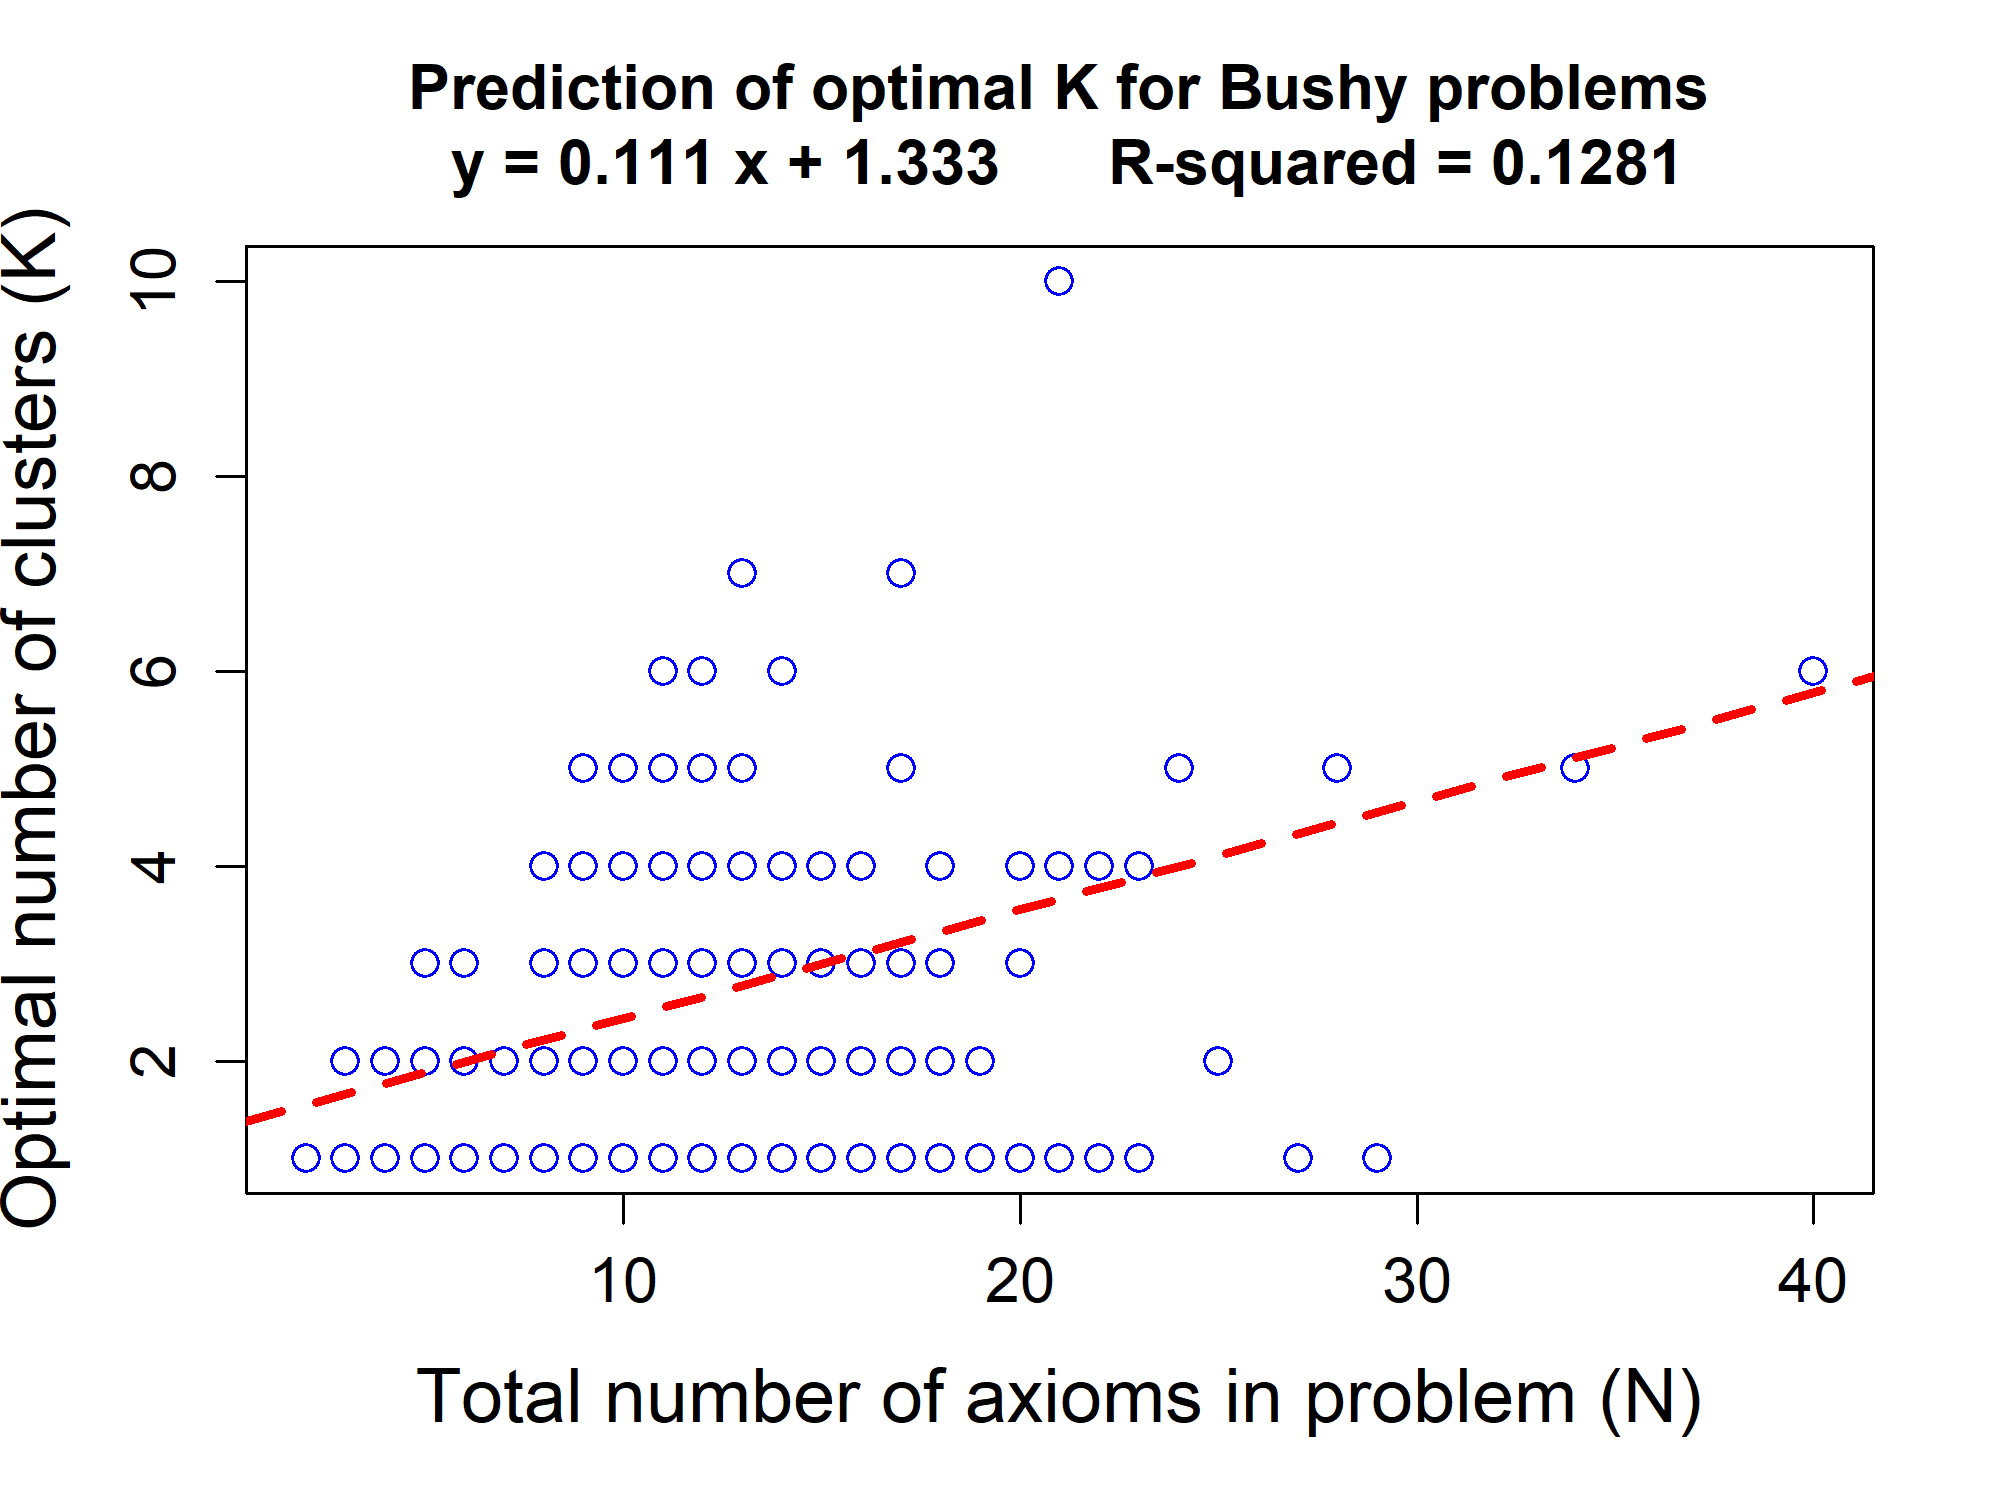
\includegraphics[scale=0.42]{median-regression-optimal-k-bushy.png}
	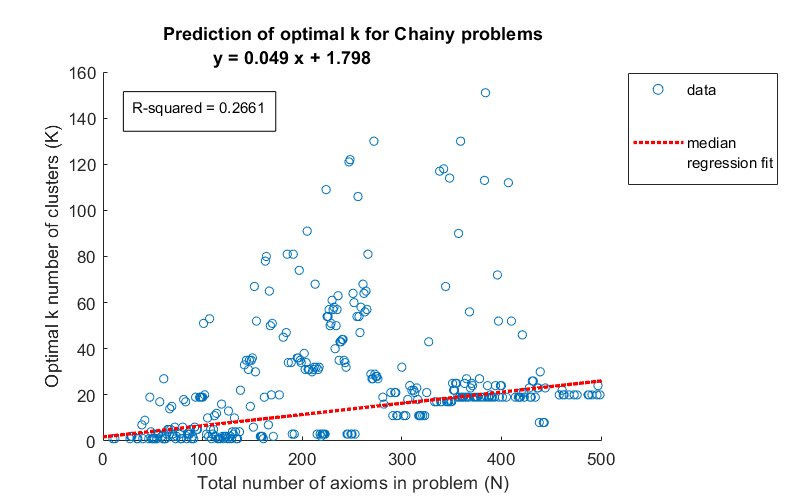
\includegraphics[scale=0.42]{median-regression-optimal-k-chainy.png}
	\vspace{1mm}
	\caption{ Median regression prediction line of $k_{best}$ as a function 
	of the total number of axioms in a problem, for Bushy problems (left) 
	and Chainy problems (right). }
	\label{fig:median-regression}
\end{figure}

%------------------------------------------------------------------------------
\subsection{Our Selection Techniques}
\label{Zihao}

4. Zihaos way
%------------------------------------------------------------------------------
\section{Evaluation Results}
\label{Results}

The new axiom selection techniques, and the axiom selection in the Vampire 
and E ATP systems, were evaluated using the metrics.
Two problems sets were used: the first was a set of 325 smaller problems
from the MPTP2078 corpus, selected by taking the chainy problems with less
that 500 axiom and for which the pruney problem exists, and the second was
the full set of 2078 problems (the smaller set was useful for initial
quick testing, and also necessary because some of the techniques took
more than the available computing resources for the full set)

Tables~\ref{Results325} and ~\ref{Results2078} show the results, including
a row for the base case in which all axioms are selected.
The columns are the 
Precision (Prcn, 
Selectivity (Sely), 
Ranking precision (RPrn), 
Ranking density (RDen), 
Adequacy (Adeq),
Adequate precision (Prcn), Adequate selectivity (Sely), Adequate
ranking precision (RPrn), and Adequate ranking density (RDen).

\begin{table}[hbt]
\begin{center}
\begin{tabular}{|l|rrrr|r|rrrr|}
\hline
Bushy problems  & \multicolumn{4}{|c|}{Average} & \multicolumn{5}{|c|}{Adequate} \\
Technique       & Prcn & Sely & RPrn & RDen & Adeq & Prcn & Sely & RPrn & RDen \\
\hline
Base            & 0.35 & 1.00 &  -   &  -   & 1.00 & 0.35 & 1.00 &  -   &  -   \\
E 2.4           & 0.35 & 1.00 &  -   &  -   & 1.00 & 0.35 & 1.00 &  -   &  -   \\
Vampire 4.4     & 0.32 & 0.80 &  -   &  -   & 0.80 & 0.39 & 0.84 &  -   &  -   \\
Q$\infty$ cut   & 0.43 & 0.54 & 0.62 & 0.52 & 0.74 & 0.58 & 0.61 & 0.84 & 0.71 \\
Spectral cl.    & 0.24 & 0.57 &  -   &  -   & 0.66 & 0.36 & 0.79 &  -   &  -   \\
Greedy path     & 0.37 & 0.77 &  -   &  -   & 0.97 & 0.38 & 0.80 &  -   &  -   \\
\hline
Chainy problems & \multicolumn{4}{|c|}{Average} & \multicolumn{5}{|c|}{Adequate} \\
Technique       & Prcn & Sely & RPrn & RDen & Adeq & Prcn & Sely & RPrn & RDen \\
\hline
Base            & 0.06 & 1.00 &  -   &  -   & 1.00 & 0.06 & 1.00 &  -   &  -   \\
E 2.4           & 0.06 & 1.00 &  -   &  -   & 1.00 & 0.06 & 1.00 &  -   &  -   \\
Vampire 4.4     & 0.08 & 0.55 &  -   &  -   & 0.94 & 0.09 & 0.56 &  -   &  -   \\
Q$\infty$ cut   & 0.08 & 0.53 & 0.57 & 0.21 & 0.85 & 0.09 & 0.56 & 0.67 & 0.25 \\
Spectral cl.    & 0.05 & 0.48 &  -   &  -   & 0.65 & 0.08 & 0.63 &  -   &  -   \\
Greedy path     & 0.05 & 0.93 &  -   &  -   & 0.96 & 0.05 & 0.96 &  -   &  -   \\
\hline
\end{tabular}
\caption{Results for the 325 smaller problems}
\label{Results325}
\end{center}
\end{table}

\begin{table}[hbt]
\begin{center}
\begin{tabular}{|l|rrrr|r|rrrr|}
\hline
Bushy problems  & \multicolumn{4}{|c|}{Average} & \multicolumn{5}{|c|}{Adequate} \\
Technique       & Prcn & Sely & RPrn & RDen & Adeq & Prcn & Sely & RPrn & RDen \\
\hline
Base            & 0.30 & 1.00 &  -   &  -   & 1.00 & 0.30 & 1.00 &  -   &  -   \\
E 2.4           & 0.30 & 1.00 &  -   &  -   & 1.00 & 0.30 & 1.00 &  -   &  -   \\
Vampire 4.4     & 0.21 & 0.69 &  -   &  -   & 0.58 & 0.36 & 0.76 &  -   &  -   \\
Q$\infty$ cut   & 0.33 & 0.54 & 0.55 & 0.42 & 0.69 & 0.48 & 0.59 & 0.81 & 0.61 \\
\hline
Chainy problems & \multicolumn{4}{|c|}{Average} & \multicolumn{5}{|c|}{Adequate} \\
Technique       & Prcn & Sely & RPrn & RDen & Adeq & Prcn & Sely & RPrn & RDen \\
\hline
Base            & 0.02 & 1.00 &  -   &  -   & 1.00 & 0.02 & 1.00 &  -   &  -   \\
E 2.4           & 0.02 & 0.98 &  -   &  -   & 1.00 & 0.02 & 0.98 &  -   &  -   \\
Vampire 4.4     & 0.03 & 0.40 &  -   &  -   & 0.87 & 0.04 & 0.41 &  -   &  -   \\
Q$\infty$ cut   & 0.03 & 0.53 & 0.46 & 0.07 & 0.83 & 0.04 & 0.56 & 0.56 & 0.08 \\
\hline
\end{tabular}
\caption{Results for all 2078 problems}
\label{Results2078}
\end{center}
\end{table}

Ade is a double edged sword.


%------------------------------------------------------------------------------
\section{Conclusion}
\label{Conclusion}

GEOFF:
1. Future correlate metrics with ptover performance (or do now!)

Make Zishi and Zihao efficient enough for 2078 testing.

%------------------------------------------------------------------------------
\label{sect:bib}
\bibliographystyle{plain}
\bibliography{Bibliography}
%------------------------------------------------------------------------------
\end{document}
%------------------------------------------------------------------------------

